\appendix
\section{Resoconto attività di verifica}\label{section:resoconto_verifica}
\subsection{Verifica dei documenti}\label{subsection:verifica_documenti}
\subsubsection{Indice di Gulpease}
\begin{figure}[H]
  \centering
  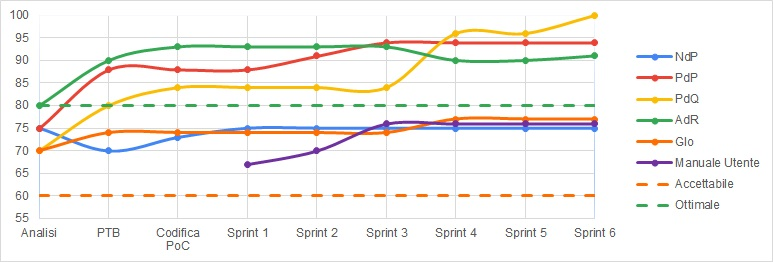
\includegraphics[scale=0.8]{immagini/gulpease.jpg}
  \caption{Indice di Gulpease di ciascun documento per periodo}
\end{figure}

\subsubsection{Errori ortografici}
\begin{figure}[H]
  \centering
  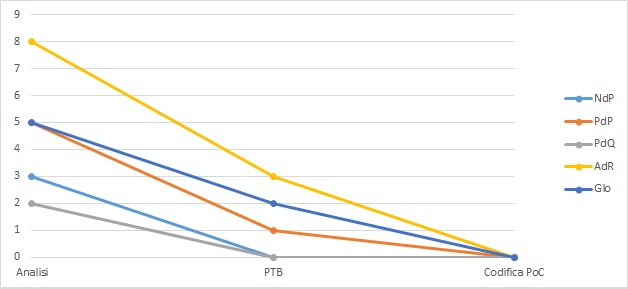
\includegraphics[scale=0.8]{immagini/err_ortografici.jpg}
  \caption{Errori ortografici individuati per periodo}
\end{figure}

%%%%%%%%%%%%%%%%%%%%%%%%%%%%%%%%%%%%%%%%%%%%%%%%%%%%%%%%%%%%%%%%%%%%%%%%%%%%%%%%%%%%%%%%%%%%%%%%

\subsection{Verifica dei processi}\label{subsection:verifica_processi}
\subsubsection{Estimated At Completion}
\begin{figure}[H]
  \centering
  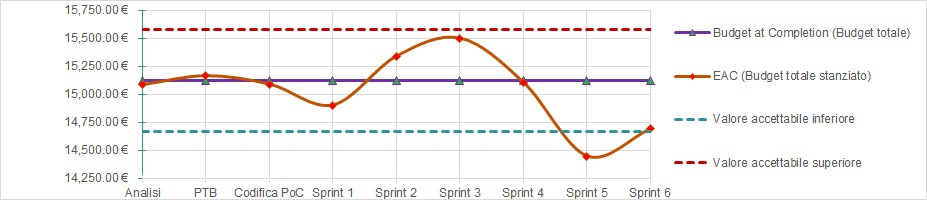
\includegraphics[scale=0.8]{immagini/eac.jpg}
  \caption{Revisione del valore stimato per la realizzazione del progetto}
\end{figure}

\subsubsection{Earned Value \& Planned Value}
\begin{figure}[H]
  \centering
  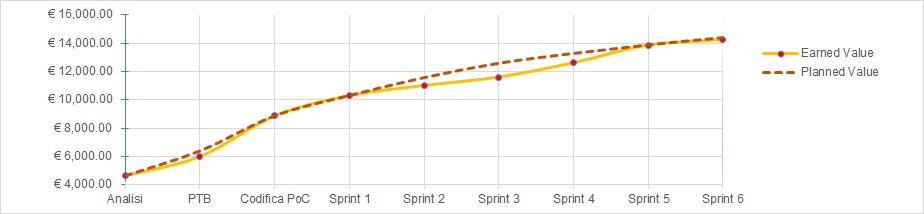
\includegraphics[scale=0.8]{immagini/ev_pv.jpg}
  \caption{Valore delle attività realizzate e costo pianificato per realizzare le rimanenti}
\end{figure}

\subsubsection{Actual Cost \& Estimate To Complete}
\begin{figure}[H]
  \centering
  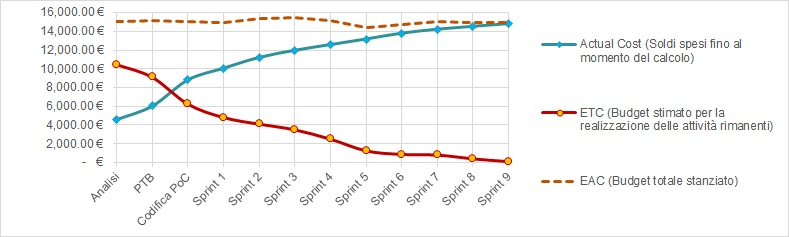
\includegraphics[scale=0.8]{immagini/ac_etc.jpg}
  \caption{Costo effettivamente sostenuto e valore stimato per la realizzazione delle rimanenti attività}
\end{figure}

\subsubsection{Schedule Variance \& Cost Variance}
\begin{figure}[H]
  \centering
  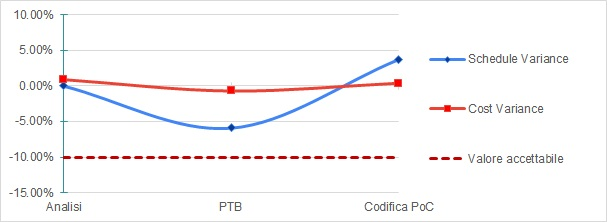
\includegraphics[scale=0.8]{immagini/sv_cv.jpg}
  \caption{Cost Variance e Schedule Variance per periodo}
\end{figure}

\subsubsection{Requirements Stability Index}
\begin{figure}[H]
  \centering
  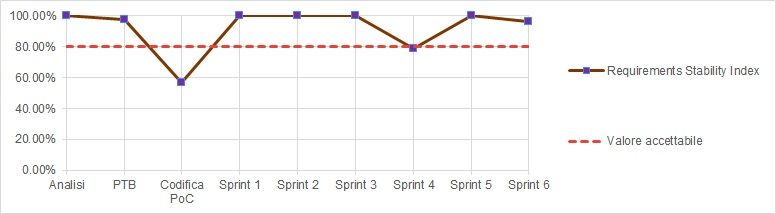
\includegraphics[scale=0.8]{immagini/rsi.jpg}
  \caption{Variazione del numero di requisiti}
\end{figure}

\subsubsection{Attualizzazione dei rischi}
\begin{figure}[H]
  \centering
  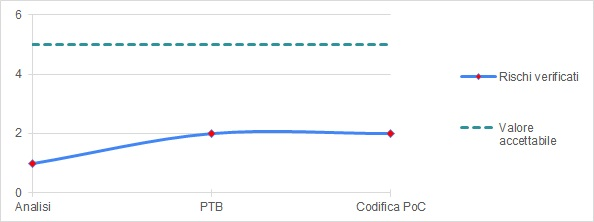
\includegraphics[scale=0.8]{immagini/rischi.jpg}
  \caption{Rischi verificati per periodo}
\end{figure}

\subsubsection{Metrics Satisfied}
\begin{figure}[H]
  \centering
  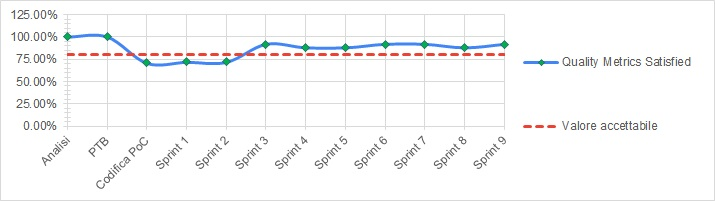
\includegraphics[scale=0.8]{immagini/metriche.jpg}
  \caption{Percentuale di metriche soddisfatte per periodo}
\end{figure}

\subsubsection{Passed Test}
\begin{figure}[H]
  \centering
  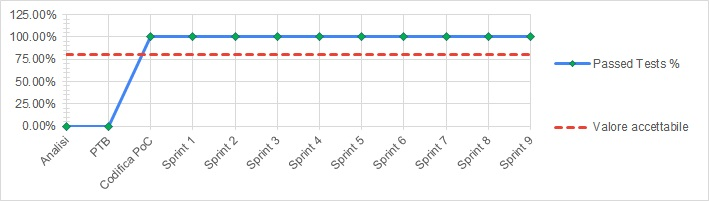
\includegraphics[scale=0.8]{immagini/tests.jpg}
  \caption{Percentuale di test passati rispetto a quelli implementati per periodo}
\end{figure}

%%%%%%%%%%%%%%%%%%%%%%%%%%%%%%%%%%%%%%%%%%%%%%%%%%%%%%%%%%%%%%%%%%%%%%%%%%%%%%%%%%%%

\subsection{Verifica dei software}\label{subsection:verifica_software}

\subsubsection{Facilità di utilizzo}
\begin{figure}[H]
  \centering
  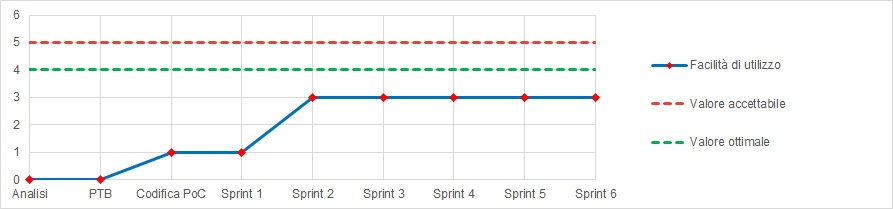
\includegraphics[scale=0.8]{immagini/facilita_utilizzo.jpg}
  \caption{Quantitativo di click necessari per raggiungere la funzione desiderata}
\end{figure}

\subsubsection{Versioni browser supportate}
\begin{figure}[H]
  \centering
  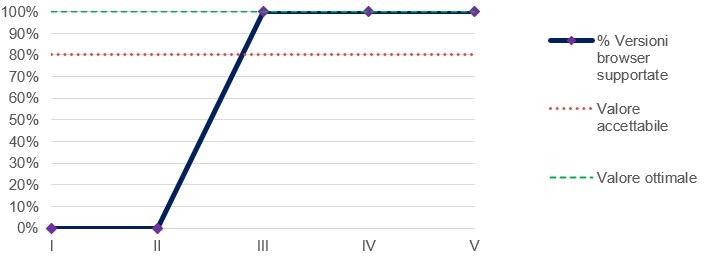
\includegraphics[scale=0.7]{immagini/browser.jpg}
  \caption{Versioni di browser supportate per periodo}
\end{figure}

\subsubsection{Copertura requisiti obbligatori}
\begin{figure}[H]
  \centering
  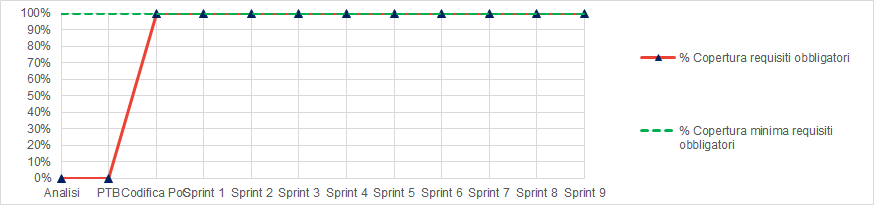
\includegraphics[scale=0.7]{immagini/cop_obbligatori.png}
  \caption{Percentuale di requisiti obbligatori implementati per periodo}
\end{figure}

\subsubsection{Copertura requisiti desiderabili}
\begin{figure}[H]
  \centering
  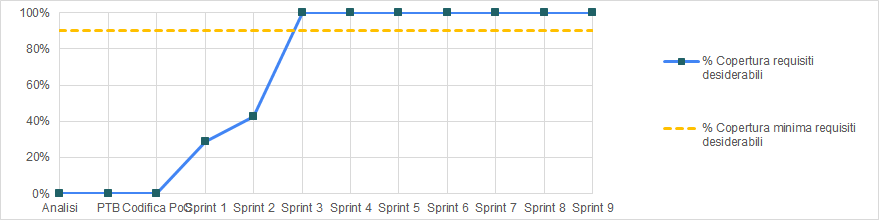
\includegraphics[scale=0.7]{immagini/cop_desiderabili.png}
  \caption{Percentuale di requisiti desiderabili implementati per periodo}
\end{figure}

\subsubsection{Copertura requisiti opzionali}
\begin{figure}[H]
  \centering
  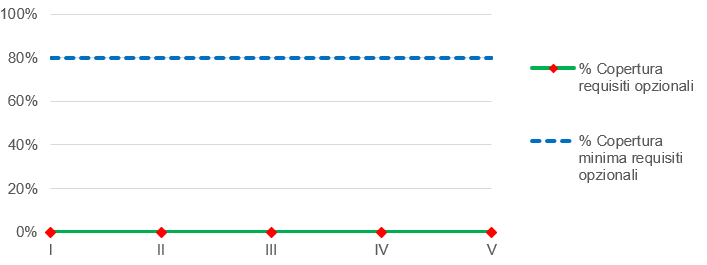
\includegraphics[scale=0.7]{immagini/cop_opzionali.png}
  \caption{Percentuale di requisiti opzionali implementati per periodo}
\end{figure}

\subsubsection{Solidity Statement Coverage}
\begin{figure}[H]
  \centering
  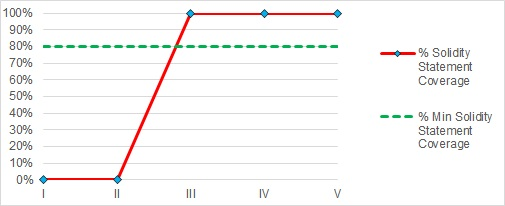
\includegraphics[scale=0.8]{immagini/solidity_statement.jpg}
  \caption{Statement Coverage riguardante il codice Solidity}
\end{figure}

\subsubsection{Solidity Branch Coverage}
\begin{figure}[H]
  \centering
  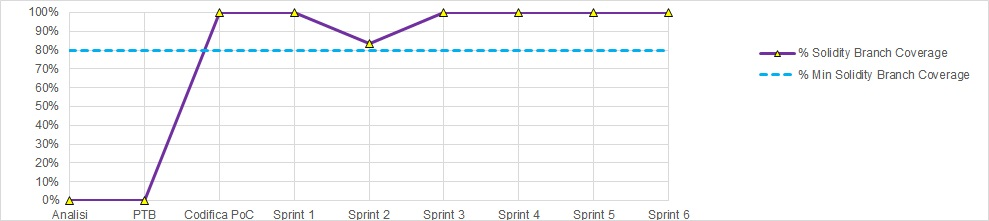
\includegraphics[scale=0.8]{immagini/solidity_branch.jpg}
  \caption{Branch Coverage riguardante il codice Solidity}
\end{figure}

\subsubsection{Solidity Function Coverage}
\begin{figure}[H]
  \centering
  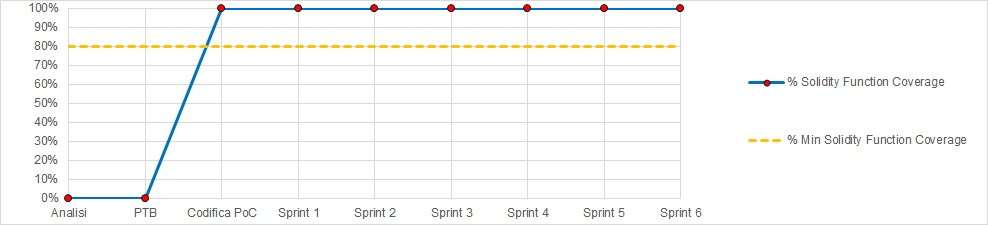
\includegraphics[scale=0.8]{immagini/solidity_function.jpg}
  \caption{Function Coverage riguardante il codice Solidity}
\end{figure}

\subsubsection{Solidity Line Coverage}
\begin{figure}[H]
  \centering
  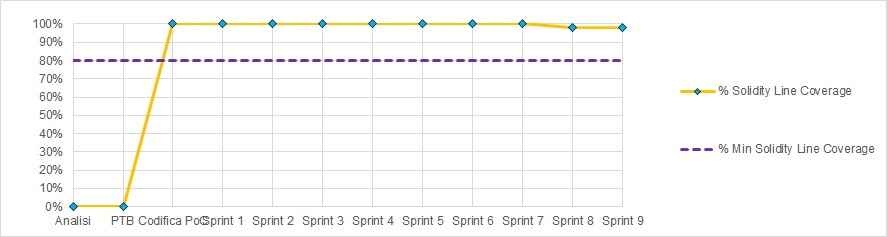
\includegraphics[scale=0.8]{immagini/solidity_line.jpg}
  \caption{Line Coverage riguardante il codice Solidity}
\end{figure}

\subsubsection{Frontend Statement Coverage}
\begin{figure}[H]
  \centering
  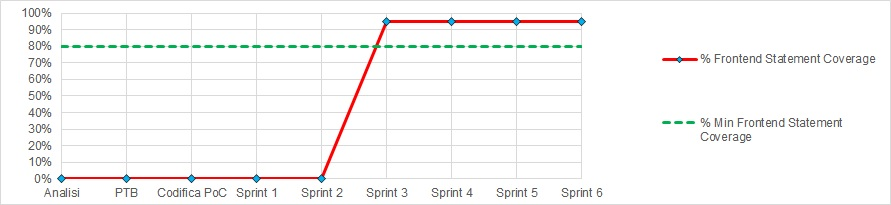
\includegraphics[scale=0.8]{immagini/frontend_statement.jpg}
  \caption{Statement Coverage riguardante il codice del frontend}
\end{figure}

\subsubsection{Frontend Branch Coverage}
\begin{figure}[H]
  \centering
  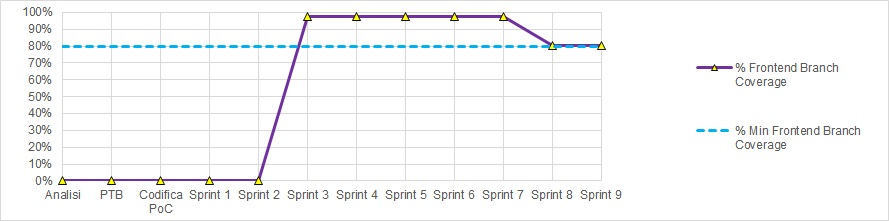
\includegraphics[scale=0.8]{immagini/frontend_branch.jpg}
  \caption{Branch Coverage riguardante il codice del frontend}
\end{figure}

\subsubsection{Frontend Function Coverage}
\begin{figure}[H]
  \centering
  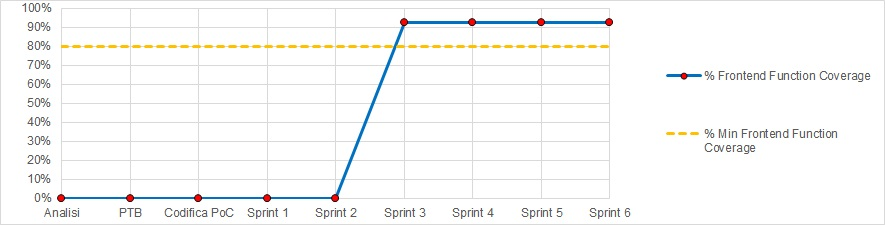
\includegraphics[scale=0.8]{immagini/frontend_function.jpg}
  \caption{Function Coverage riguardante il codice del frontend}
\end{figure}

\subsubsection{Frontend Line Coverage}
\begin{figure}[H]
  \centering
  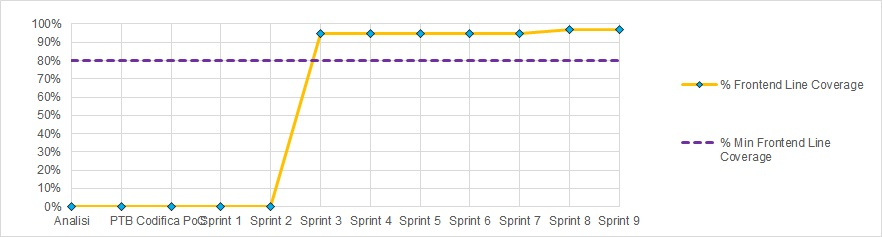
\includegraphics[scale=0.8]{immagini/frontend_line.jpg}
  \caption{Line Coverage riguardante il codice del frontend}
\end{figure}